	% v2-acmsmall-sample.tex, dated March 6 2012
% This is a sample file for ACM small trim journals
%
% Compilation using 'acmsmall.cls' - version 1.3 (March 2012), Aptara Inc.
% (c) 2010 Association for Computing Machinery (ACM)
%
% Questions/Suggestions/Feedback should be addressed to => "acmtexsupport@aptaracorp.com".
% Users can also go through the FAQs available on the journal's submission webpage.
%
% Steps to compile: latex, bibtex, latex latex
%
% For tracking purposes => this is v1.3 - March 2012

\documentclass[prodmode,acmtecs]{acmsmall} % Aptara syntax

% Package to generate and customize Algorithm as per ACM style
\usepackage[ruled]{algorithm2e}


%%%ADDED%%%%%
\usepackage{graphicx}


\graphicspath{{images/}}
\usepackage{url}
%\usepackage{biblatex}
\usepackage{color}
\usepackage{listings}
\usepackage{tabularx} 
\usepackage{ragged2e}
\usepackage{xcolor,colortbl}
\usepackage{multirow}
\usepackage{subfigure}
%\usepackage[numbers,sort&compress,square]{natbib}
\usepackage[noadjust]{cite}
%\usepackage{algorithm}
%\usepackage[noend]{algpseudocode}

\usepackage[utf8]{inputenc}
\usepackage{cleveref}
\crefname{section}{§}{§§}
\Crefname{section}{§}{§§}
\usepackage[shortcuts]{extdash} 
\usepackage{balance}
\usepackage{csvsimple}


\usepackage[utf8]{inputenc}

\pagenumbering{arabic}


\newcommand{\Fix}[1]{\textcolor{red}{[#1]}}

\newcommand{\borrowed}[1]{\textcolor{blue}{[#1]}}

%%%%End ADDED%%%%
\renewcommand{\algorithmcfname}{ALGORITHM}
\SetAlFnt{\small}
\SetAlCapFnt{\small}
\SetAlCapNameFnt{\small}
\SetAlCapHSkip{0pt}
\IncMargin{-\parindent}

% Metadata Information
\acmVolume{9}
\acmNumber{4}
\acmArticle{39}
\acmYear{2010}
\acmMonth{3}

% Copyright
%\setcopyright{acmcopyright}
%\setcopyright{acmlicensed}
%\setcopyright{rightsretained}
%\setcopyright{usgov}
%\setcopyright{usgovmixed}
%\setcopyright{cagov}
%\setcopyright{cagovmixed}

% DOI
\doi{0000001.0000001}

%ISSN
\issn{1234-56789}

% Document starts
\begin{document}
% Page heads
\markboth{XX et al.}{Building Blocks of Large Scale Stream Processing: the Past, Current, and Future}

% Title portion
\title{Building Blocks of Large Scale Stream Processing: the Past, Current, and Future}
\author{
XX
\affil{UIUC}
YY
\affil{UIUC}
}


\begin{abstract}
	\Fix{TODO
		chicken chicken chicken :D}
\end{abstract}


%
% The code below should be generated by the tool at
% http://dl.acm.org/ccs.cfm
% Please copy and paste the code instead of the example below. 
%

\begin{CCSXML}
	<ccs2012>
	<concept>
	<concept_id>10010520.10010553.10010562</concept_id>
	<concept_desc>Computer systems organization~Embedded systems</concept_desc>
	<concept_significance>500</concept_significance>
	</concept>
	<concept>
	<concept_id>10010520.10010575.10010755</concept_id>
	<concept_desc>Computer systems organization~Redundancy</concept_desc>
	<concept_significance>300</concept_significance>
	</concept>
	<concept>
	<concept_id>10010520.10010553.10010554</concept_id>
	<concept_desc>Computer systems organization~Robotics</concept_desc>
	<concept_significance>100</concept_significance>
	</concept>
	<concept>
	<concept_id>10003033.10003083.10003095</concept_id>
	<concept_desc>Networks~Network reliability</concept_desc>
	<concept_significance>100</concept_significance>
	</concept>
	</ccs2012>  
\end{CCSXML}

\ccsdesc[500]{Computer systems organization~Embedded systems}
\ccsdesc[300]{Computer systems organization~Redundancy}
\ccsdesc{Computer systems organization~Robotics}
\ccsdesc[100]{Networks~Network reliability}

%
% End generated code
%

% We no longer use \terms command
%\terms{Design, Algorithms, Performance}

\keywords{\Fix{todo}}

%\acmformat{Gang Zhou, Yafeng Wu, Ting Yan, Tian He, Chengdu Huang, John A. Stankovic,
%	and Tarek F. Abdelzaher, 2010. A multifrequency MAC specially
%	designed for  wireless sensor network applications.}
% At a minimum you need to supply the author names, year and a title.
% IMPORTANT:
% Full first names whenever they are known, surname last, followed by a period.
% In the case of two authors, 'and' is placed between them.
% In the case of three or more authors, the serial comma is used, that is, all author names
% except the last one but including the penultimate author's name are followed by a comma,
% and then 'and' is placed before the final author's name.
% If only first and middle initials are known, then each initial
% is followed by a period and they are separated by a space.
% The remaining information (journal title, volume, article number, date, etc.) is 'auto-generated'.

\begin{bottomstuff}
%	This work is supported by the National Science Foundation, under
%	grant CNS-0435060, grant CCR-0325197 and grant EN-CS-0329609.
%	
%	Author's addresses: G. Zhou, Computer Science Department,
%	College of William and Mary; Y. Wu  {and} J. A. Stankovic,
%	Computer Science Department, University of Virginia; T. Yan,
%	Eaton Innovation Center; T. He, Computer Science Department,
%	University of Minnesota; C. Huang, Google; T. F. Abdelzaher,
%	(Current address) NASA Ames Research Center, Moffett Field, California 94035.
\end{bottomstuff}

\maketitle
\section{Introduction}
\label{sec:intro}

In the era of Big Data, humongous amount of data is produced every second from diverse sources such as social networks, sensors, IoT, etc. In majority of use-cases, processing this massive amount of data  is latency sensitive (sub-seconds to minutes), either because of  cost benefits (e.g., every second latency in Google cost \Fix{X}) or the need for a critical action (e.g., detecting attacks and reacting to it).

To address this need, many Stream Processing systems have been developed with the ability of processing huge amount of data on a distributed cluster of machines in a near real-time fashion \Fix{cite}.  




\begin{table}[h]
	%\centering
	\tbl{Essential building blocks in Stream Processing Engines.	\label{blocks-table}}{
\begin{tabular}{|l|l|}%
	\hline
	\rowcolor[HTML]{E0E0E0} 
	\bfseries Building Block & \bfseries % specify table head
	\csvreader[head to column names]{tables/building-blocks.csv}{}% use head of csv as column names
	{\\\hline\csvcoli&\csvcolii}% specify your coloumns here
	\\ \hline
\end{tabular}
}
\end{table}




\section{Stream Processing and its Building blocks}

\subsection{Background}

\begin{itemize}
	\item basic definitions of stream processing. 
	\item what is operator
	\item how do messages flow
	\item how operators are connected
	\item API
\end{itemize}


\subsection{High Level Overview}
\begin{itemize}
	\item describe the main building blocks. These are in Table \ref{table:blocks}
	\item discuss the definition, purpose, importance of each block.	
\end{itemize}


\begin{table}[h]
	%\centering
	\tbl{Essential building blocks in Stream Processing Engines.	\label{table:blocks}}{
		\begin{tabular}{c|l|l}%
			\hline
			\rowcolor[HTML]{E0E0E0} 
			\bfseries Section & \bfseries Building Block & \bfseries Definition  % specify table head
			\csvreader[head to column names]{tables/building-blocks.csv}{}% use head of csv as column names
			{\\\hline\csvcoli&\csvcolii & \csvcoliii}% specify your coloumns here
			\\ \hline
		\end{tabular}
	}
\end{table}

\Fix{Do we want to argue we are covering all essential building blocks??? or just say the most important ones?}




\subsection{Interaction Among Building Blocks}

\begin{itemize}
	\item Draw a figure of the building blocks and their interaction. 
	\item Talk about how the influence each other
	\item Maybe try to break them down into a layers? with some being in a touching-all layer?
\end{itemize}


%

\begin{figure}[h]
	\centering
	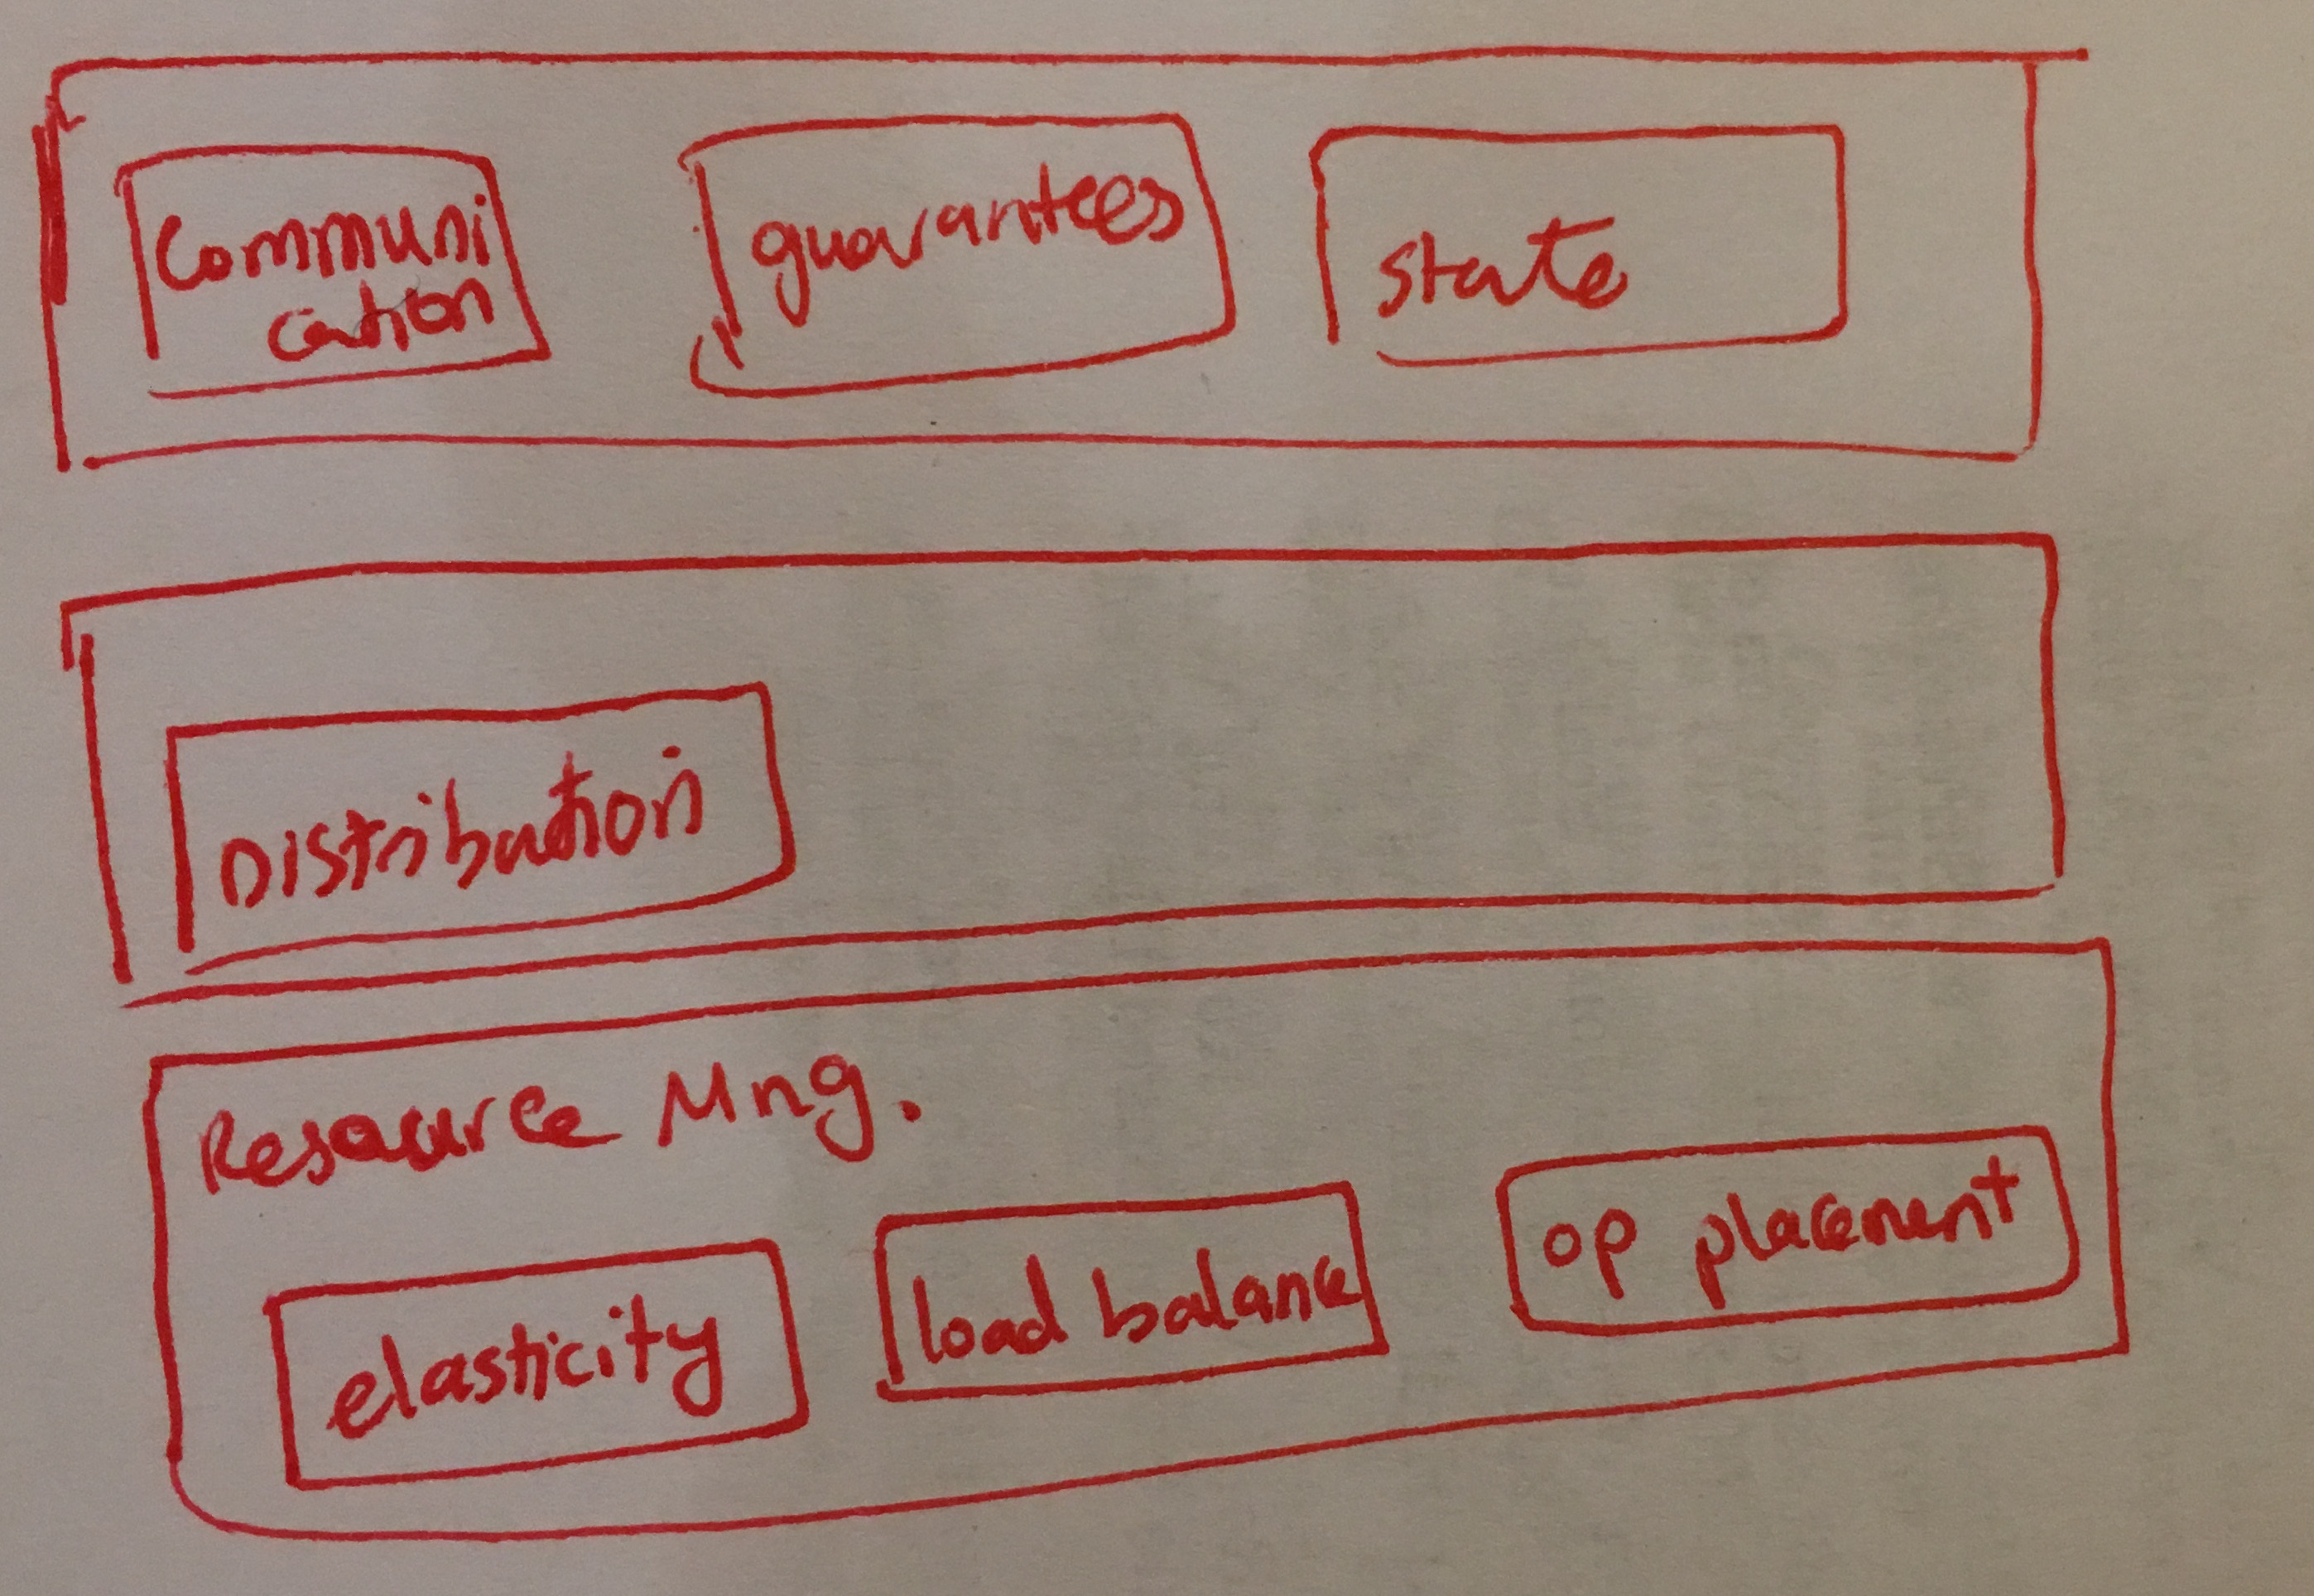
\includegraphics[width=0.45\linewidth]{interaction.jpg}
	\caption{\Fix{Sample figure of how components interact with one another. This is not complete.}}
	\label{fig:tree-cpVScl}
\end{figure}





%%%%%%%%% BUILDING BLOCKS %%%%%%%%%%
\section{Parallelization, Distribution, and Grouping}
\label{sec:parallelization}

\subsection{Parallelization}
 To handle large scale, processing has to be done in parallel and distributed among many machines. Thus, Stream processing systems break applications and streams into smaller units. An application is composed of many independent operators, and each operator has several parallel instances (Figure \ref{fig:stream}). Similarly, a stream is composed of several \textit{partitions}. Figure \ref{fig:parallelization}-a shows an example dataflow with partitions $\{P_{AB}\_1, P_{AB}\_2, P_{AB}\_3\}$. \Fix{how about when they all have similar duplicate input?}
Each instance autonomously operators on a separate partition of the input stream (e.g., $B_1$ on $P_{AB}\_1$), and produces output to partitions of an output stream (e.g., $A_1$ outputting to all partitions ). 

\subsection{Distribution}
Stream applications are distributed across a cluster of processing \textit{nodes}, as shown in Figure \ref{fig:parallelization}-b. Typically, each instance is treated as a single thread \footnote{Some systems use a different variation of instance to thread mapping. For example, Storm enables mapping multiple instances to a thread, and Samza used to provide a single thread (per process) model \Fix{cite}.}. 
Instances are placed together into a \textit{process} or container (which is essentially a process), and then processes are distributed across nodes. Note that in a given node, process of a given application or two different applications may run concurrently. 
Section \Fix{X and Y} discuss the different placement and distribution strategies used for both instances and processes. 
\Fix{should this be here? or move to another section}
	
\begin{figure}[t]
	\centering
	\subfigure[Parallelization and partitioning]{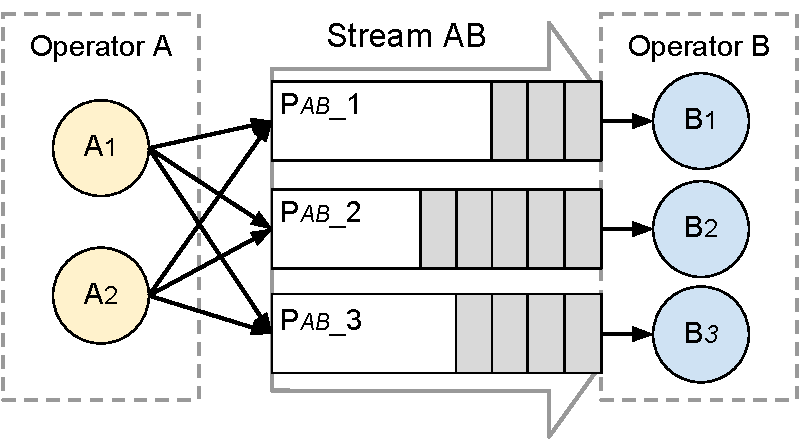
\includegraphics[width=0.45\linewidth]{partition}}
	\hspace*{1cm}
	\subfigure[Distribution]{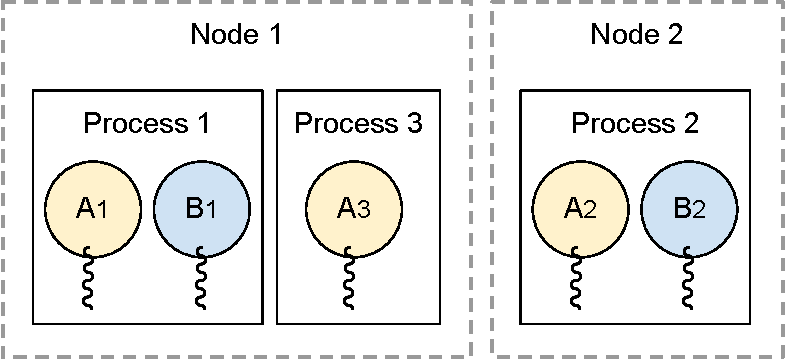
\includegraphics[width=0.45\linewidth]{distibution} 
	}
	\caption{An example application with two operators, A and B, with: a) the parallelization of operators into instances (A = $\{A_1, A_2\}$, B =$\{B_1, B_2, B_3\}$) and partitioning of the AB Stream, and b) the distribution of instances among processing nodes.}
\label{fig:parallelization}
	
\end{figure}

\subsection{Grouping}

\noindent \textbf{Definition:} As shown in Figure \ref{fig:parallelization}-a, an operator instance ($A_1$) outputs items to all partitions of an output stream. The \textit{grouping} strategy defines which partition(s) an output item should be added to. Grouping are defined per stream. An operator with various input streams might have different grouping in each.

\noindent \textbf{\\Solutions, trade-offs and usecases:}
For a given instance $o_s$ of $O_{src}$ generating item $i$ to $O_{dst}$, through output stream $s$ with partitions $P_s=\{p_1, p_2, ..., p_k\}$, the common groupings are:
\begin{itemize}
	\item \textbf{Random:} where $i$ is randomly assigned to one of the partitions in $P_s$. Random grouping guarantees load balance among partitions in terms of number of items. However, this approach is unaware of the placement of instances (locality unaware). This grouping is one of the most common groupings.
	\item \textbf{Hash-based:} where using a consistent hashing on the item's key, $i$ is hashed to one of the partitions in $P_s$. \Fix{define item's key}. This grouping guarantees all items with the same key go to the same partition (thus, processed by one instance). This is a commonly used grouping and necessary feature when doing joins or aggregations over a specific key. However, poor hashing and skewed data can create load imbalance.
	
	\Fix{@ le: there is another mode of hash-based (Partial Key grouping: ) along with load balancing. I think it belongs to the load balancing section or should be removed entirely. it is based on this paper:
	https://melmeric.files.wordpress.com/2014/11/the-power-of-both-choices-practical-load-balancing-for-distributed-stream-processing-engines.pdf	
	}

	\item \textbf{All:} where $i$ is replicated and sent to \textit{all} partitions. This grouping acts as a broadcast, and should be used with care because of its high overhead. This is mostly useful for sending coordination and management messages.
	\item \textbf{One:} where all items, such as $i$,  are sent to one specific partition, e.g, $p_1$. This is mostly used when all data needs to be aggregated at one processor. However, it create huge load-imbalance. This is a special case of Hash-based grouping.
	\item \textbf{Locality aware:} where placement of instances are considered in sending $i$. If an instance $o_d$ of $O_{dst}$ is placed on the same process as where $o_s$ is placed, $i$ is sent to $o_d$. Otherwise, a random instance of $O_{dst}$ is chosen. This approach minimizes network traffic and latency. However poor placements can create load imbalance.


	

	Local or shuffle grouping: If the target bolt has one or more tasks in the same worker process, tuples will be shuffled to just those in-process tasks. Otherwise, this acts like a normal shuffle grouping.
\end{itemize}

Stream processing frameworks mostly support all these groupings. Table \ref{table:grouping} summarizes the groupings, their trade-offs, and the systems providing them.

\begin{table}[h]
	\tbl{Grouping solutions and their trade-offs	\label{table:grouping}}{
		\tiny		
		\begin{tabular}{p{.1 \linewidth}|p{.2 \linewidth}|p{.45 \linewidth}|p{0.07 \linewidth}}%
			
			\hline
			\rowcolor[HTML]{E0E0E0} 
			Solution	&Description&Trade-offs & Usecase
			\csvreader[head to column names]{tables/grouping.csv}{}% use head of csv as column names
			{\\\hline\textbf{\csvcoli} & \csvcolii & \csvcoliii & \csvcoliv}% specify your coloumns here
			\\ \hline
		\end{tabular}	
	}
\end{table}



\noindent \textbf{\\Future Direction:}  
\Fix{is there any?}
\section{Communication Mechanism}
\label{sec:communication}


\noindent\textbf{Definition and Purpose:} To enable large scale processing, operators are distributed across multiple machines. This distribution necessitates a \textit{communication mechanism} connecting operators to each other, and enabling data items to flow between operators. This section covers the desired properties from the communication mechanism and the current technologies used.



\noindent \textbf{\\Properties:}
%Various communicatStream processing frameworks utlize diverse comminucation mechanism based on properties they require from the communication
%
Among the various communication mechanism \Fix{cite}, the main differentiator is the properties and guarantees they provide. 
Based on these properties, stream processing frameworks employ the mechanism that best fits their requirements. The main properties of a communication mechanism are:

\begin{itemize}
	
	
	\item \textbf{Push/Pull} Which direction initiates communication? The sender can push the items downstream, the receiver can pull from upstream, or a mixed push-pull approach can be used, such as a publish-subscribe mechanism. \Fix{cite}
	
	
	\item \textbf{Fault-tolerance:} Can the mechanism handle failures? In presence of a failure, is availability impacted or can data get lost? \Fix{is this a valid point? should it be here?}
	\item \textbf{Replayability}: Can the message be replayed? If so, for how far in the past and how large is the buffer?
	%\item \textbf{buffering: } are there any buffering capabilities. How large is the buffer?
	
	\item \textbf{Ordering:} Are there any ordering guarantees, such as total ordering,  first in first out (FIFO) or 
	
	\item \textbf{ direct or proxy}: is the communication direct from one machine to another or through a second entity?
	\item \textbf{ batch or online: } is the communication done in batches or sent as soon as available?
\end{itemize}

\noindent \textbf{\\Solutions, trade-offs and usecases:}

\begin{itemize}
	\item RPC methods
	\item publish-subscribe through 3rd entity (kafka)
	\item direct pub-sub. -- zeroMQ
	\Fix{TODO: study this in more detail}
	
\end{itemize}



\noindent \textbf{\\Future Direction:}  
.





\section{Message Failure Handling}

	\noindent\textbf{Definition:} 

	\noindent \textbf{Purpose:} This BB adds guarantees to the processing. Also, provides a mean to trade-off between performance and precise computing. As shown in \ref{fig:guarantees}, "at-most-once provides higher performance with lower latency and higher throughput, with more overhead being added as moving to "exactly-once". However, this comes at a cost of less precise processing with the possibility of loosing messages or processing the same message multiple times.
	
	\noindent \textbf{Properties}
	we have three modes of guarantees 
	\begin{itemize}
		\item at most once (weakest) : guaranteeing each message is processed at most once with a chance of getting lost
		\item at least once: guaranteeing processing each message at least once, with a chance of reprocessing some of the messages
		\item exactly once (strongest): guaranteeing each message being processed exactly one (no loss or reprocessing)
	\end{itemize}	 
	\begin{figure}[h]
		\centering
		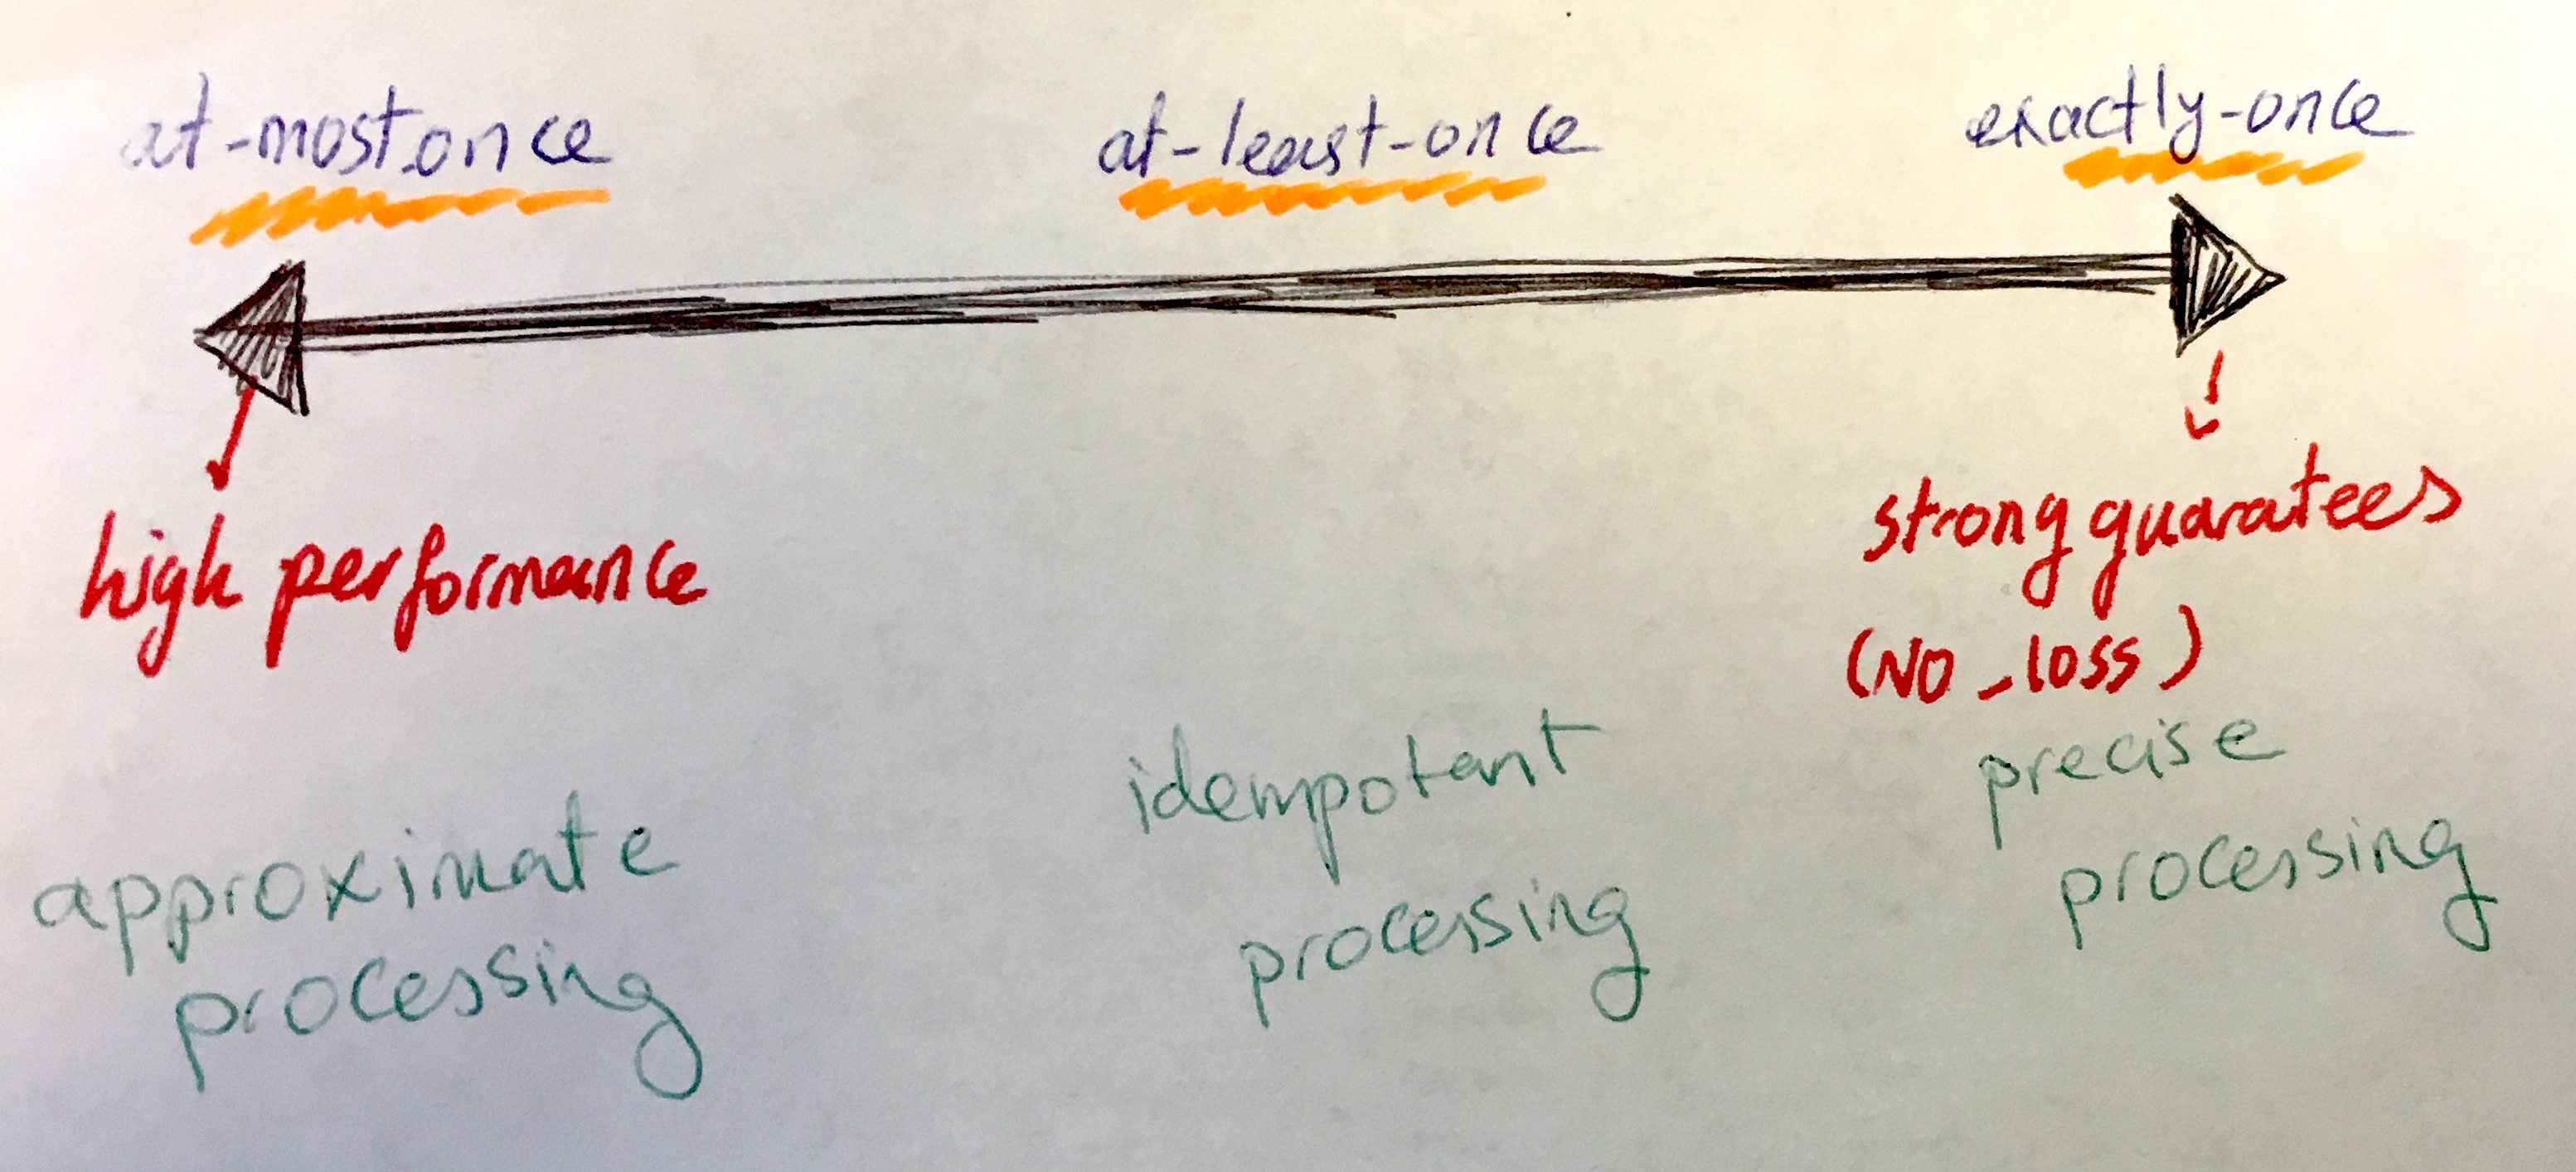
\includegraphics[width=0.45\linewidth]{guarantees.jpg}
		\caption{Spectrum of various guarantees and the trade-off among them.}
		\label{fig:guarantees}
	\end{figure}
	
	at-most-once is good for approximate computing. Examples are: \Fix{...}. at-least-once is good for idempotent computations. in most cases ordering is preserved, and a series of messages are replayed. \Fix{is that true?}. Examples are: \Fix{...}.  exactly-once is good for cases that precise computation is needed. Examples are: \Fix{...}\\
	

\noindent \textbf{Solutions \& trade-offs:} at-most once, essentially means not adding any feature to the system. at-least once mechanism are: 1. using an (XOR based) acking. 2. using ordered messaging, with latest offset processed and replay when ever missing. 3. ?

exactly-once mechanism: 1. keeping track of all message ids processed, and check before reprocessing. 2. using total ordering, and detecting missing messages and re-requesting them 
\Fix{TODO: complete the selections} \\

\begin{table}[h]
	%\centering
	\tbl{Solutions to providing streaming gurantees and their trade-offs	\label{table:msg-fault-summary}}{
		%		\begin{tabular}{|p{.1 \linewidth}|p|p|p|p|p|p|p|p|p|p|p|p|}%
		\tiny
		%	\begin{tabular}{|p{.09 \linewidth}|p{.05 \linewidth}|p{.05 \linewidth}|p{.05 \linewidth}|p{.05 \linewidth}|p{.05 \linewidth}|
		%	p{.05 \linewidth}|p{.05 \linewidth}|p{.05 \linewidth}|p{.05 \linewidth}|p{.05 \linewidth}|p{.05 \linewidth}|p{.05 \linewidth}|}%
		
		\begin{tabular}{|p{.1 \linewidth}|p{.12 \linewidth}|p{.3 \linewidth}|p{.3 \linewidth}|p{.08 \linewidth}|}%
			
			\hline
			\rowcolor[HTML]{E0E0E0} 
			Feature	&Solution	&Pros&Cons & Usecase
			\csvreader[head to column names]{tables/msg-fault-summary.csv}{}% use head of csv as column names
			{\\\hline\textbf{\csvcoli} & \csvcolii & \csvcoliii &\csvcoliv & \csvcolv }% specify your coloumns here
			\\ \hline
		\end{tabular}	
	}
\end{table}

 
\noindent \textbf{Future Direction:} current exactly once mechanism introduce too much overhead, especially in a system with high throughput. It is desirable to build a lower overhead mechanism. 







\section{Failure Detection, Tolerance, and Recovery}
\label{sec:fault}


\noindent\textbf{Definition:} 
	We have three modes of recovery:
\begin{itemize}
	
	\item  Precise recovery 
	\item  Rollback recovery
	\item Gap recovery
	\Fix{draw a similar diagram to guarantees for this?}
\end{itemize}

\noindent \textbf{\\Purpose:} 

Failures are the norm. there is a need for a component to detect and recover from failures. since stream jobs are every running jobs, this is an essential component. different modes, provide different guarantees.

\noindent \textbf{\\Use-case:}

	\begin{itemize}
	\item precise recovery:  \borrowed{hides the effects of a failure perfectly, except
		for some transient increase in processing latency, and is
		well-suited for applications that require the post-failure output
		be identical to the output without failure. Many financial
		services applications have such strict correctness requirements.}
	\item rollback recovery: \borrowed{ avoids information loss without guaranteeing
	precise recovery. The output produced after a failure
	is “equivalent” to, but not necessarily the same as, the
	output of an execution without failure. The output may also
	contain duplicate tuples. To avoid information loss, the system
	must preserve all the necessary input data for the backup
	server to rebuild (from its current state) the primary’s state at
	the moment of failure. Rollback recovery is thus appropriate
	for applications that cannot tolerate information loss but
	may tolerate imprecise output caused by the backup server
	reprocessing the input somewhat differently than the primary
	did. Example applications include those that monitor specific
	conditions (e.g., fire alarms, theft prevention through asset
	tracking). We show in Section 6 that this recovery guarantee
	can be provided more efficiently than precise recovery both
	in terms of runtime overhead and recovery speed.}
	\item gap recovery: \borrowed{ our weakest recovery guarantee, addresses
	the needs of applications that operate solely on the most recent
	information (e.g., sensor-based environment monitoring),
	where dropping some old data is tolerable for reduced
	recovery time and runtime overhead}
	\end{itemize}


\noindent \textbf{\\Solutions \& trade-offs:}

\borrowed{ employs a different combination of redundant
	computation, checkpointing, and remote logging, they offer
	different tradeoffs between runtime overhead and recovery
	performance.
}
\begin{itemize}
	\item \borrowed{all following items borrowed!}
	\item amnesia, a lightweight scheme that provides
	\textbf{gap} recovery without any runtime overhead (Section 4).
	\item  passive standby and active standby, two
	process-pairs [4, 10] approaches tailored to stream processing.
	In passive standby, each primary server (a.k.a. node) periodically
	reflects its state updates to its secondary node. In
	active standby, the secondary nodes process all tuples in parallel
	with their primaries. 
	\item  propose upstream backup,
	an approach that significantly reduces runtime overhead compared
	to the standby approaches while trading off a small
	fraction of recovery speed. 
	
	Last two items can be both roll-back and precise recovery.
	
	\Fix{are there other approaches?}
\end{itemize}


\begin{table}[h]
	\tbl{Solutions to \Fix{XXX} and their trade-offs	\label{table:failure-summary}}{
		\tiny		
		\begin{tabular}{p{.15 \linewidth}|p{.3 \linewidth}|p{.3 \linewidth}|p{.1 \linewidth}}%
			
			\hline
			\rowcolor[HTML]{E0E0E0} 
			Solution	&Pros&Cons & Usecase
			\csvreader[head to column names]{tables/template-summary.csv}{}% use head of csv as column names
			{\\\hline\textbf{\csvcoli} & \csvcolii & \csvcoliii & \csvcoliv}% specify your coloumns here
			\\ \hline
		\end{tabular}	
	}
\end{table}


\noindent \textbf{\\Future Direction:}  

\Fix{TODO}





\Fix{Should  detection,  tolerance and recovery be separated?}

\Fix{How about high availability?}
\section{Accuracy: Handling late and out-of-order messages}
\section{Handling State}
\label{sec:state}

\begin{itemize}
	\item  Stateless
	\item  Remote Storage
	\item  Local Store
	\item  case: In-mem
	\item case: On-disk
	
\end{itemize}

Things needed: 
\noindent\textbf{Definition:} 

\noindent \textbf{\\Purpose:} 


\noindent \textbf{\\Properties:}

\noindent \textbf{\\Solutions, trade-offs and usecases:}

\begin{table}[h]
	\tbl{Solutions to \Fix{XXX} and their trade-offs	\label{table:XXX-summary}}{
		\tiny		
		\begin{tabular}{p{.15 \linewidth}|p{.3 \linewidth}|p{.3 \linewidth}|p{.1 \linewidth}}%
			
			\hline
			\rowcolor[HTML]{E0E0E0} 
			Solution	&Pros&Cons & Usecase
			\csvreader[head to column names]{tables/template-summary.csv}{}% use head of csv as column names
			{\\\hline\textbf{\csvcoli} & \csvcolii & \csvcoliii & \csvcoliv}% specify your coloumns here
			\\ \hline
		\end{tabular}	
	}
\end{table}


\noindent \textbf{\\Future Direction:}  


\Fix{Fault-tolerance of state is a separate discussion}
\section{Replaying and Reprocessing}

many case need to reprocess an entire or part of the stream. this could be due to buisness logic changes or failure and so on. There needs to be a mechanism to rollback and reply. This can be done through the communication or through upstream or the processing component and so on.

\section{Flexibility and Dynamicity}
\section{Job Optimizations}
\section{Scheduling Operators}
\section{Resource Management}
\section{Resource Management}
\label{sec:resource}

\noindent \textbf{\\Purpose:} 

Failures are the norm. there is a need for a component to detect and recover from failures. since stream jobs are every running jobs, this is an essential component. different modes, provide different guarantees.

\subsection{Failure Detection}
\Fix{maybe talk about heartbeat, pingpong, or piggy back mechanisms?}
\subsection{Failure Tolerance}
\Fix{talk about mechanism used for availability. Maybe the independent design structure that one some of the paths are unavailable not the whole dataflow.}
\subsection{Failure Recovery}

\noindent \textbf{\\Properties:}


\begin{figure}[h]
	\centering
	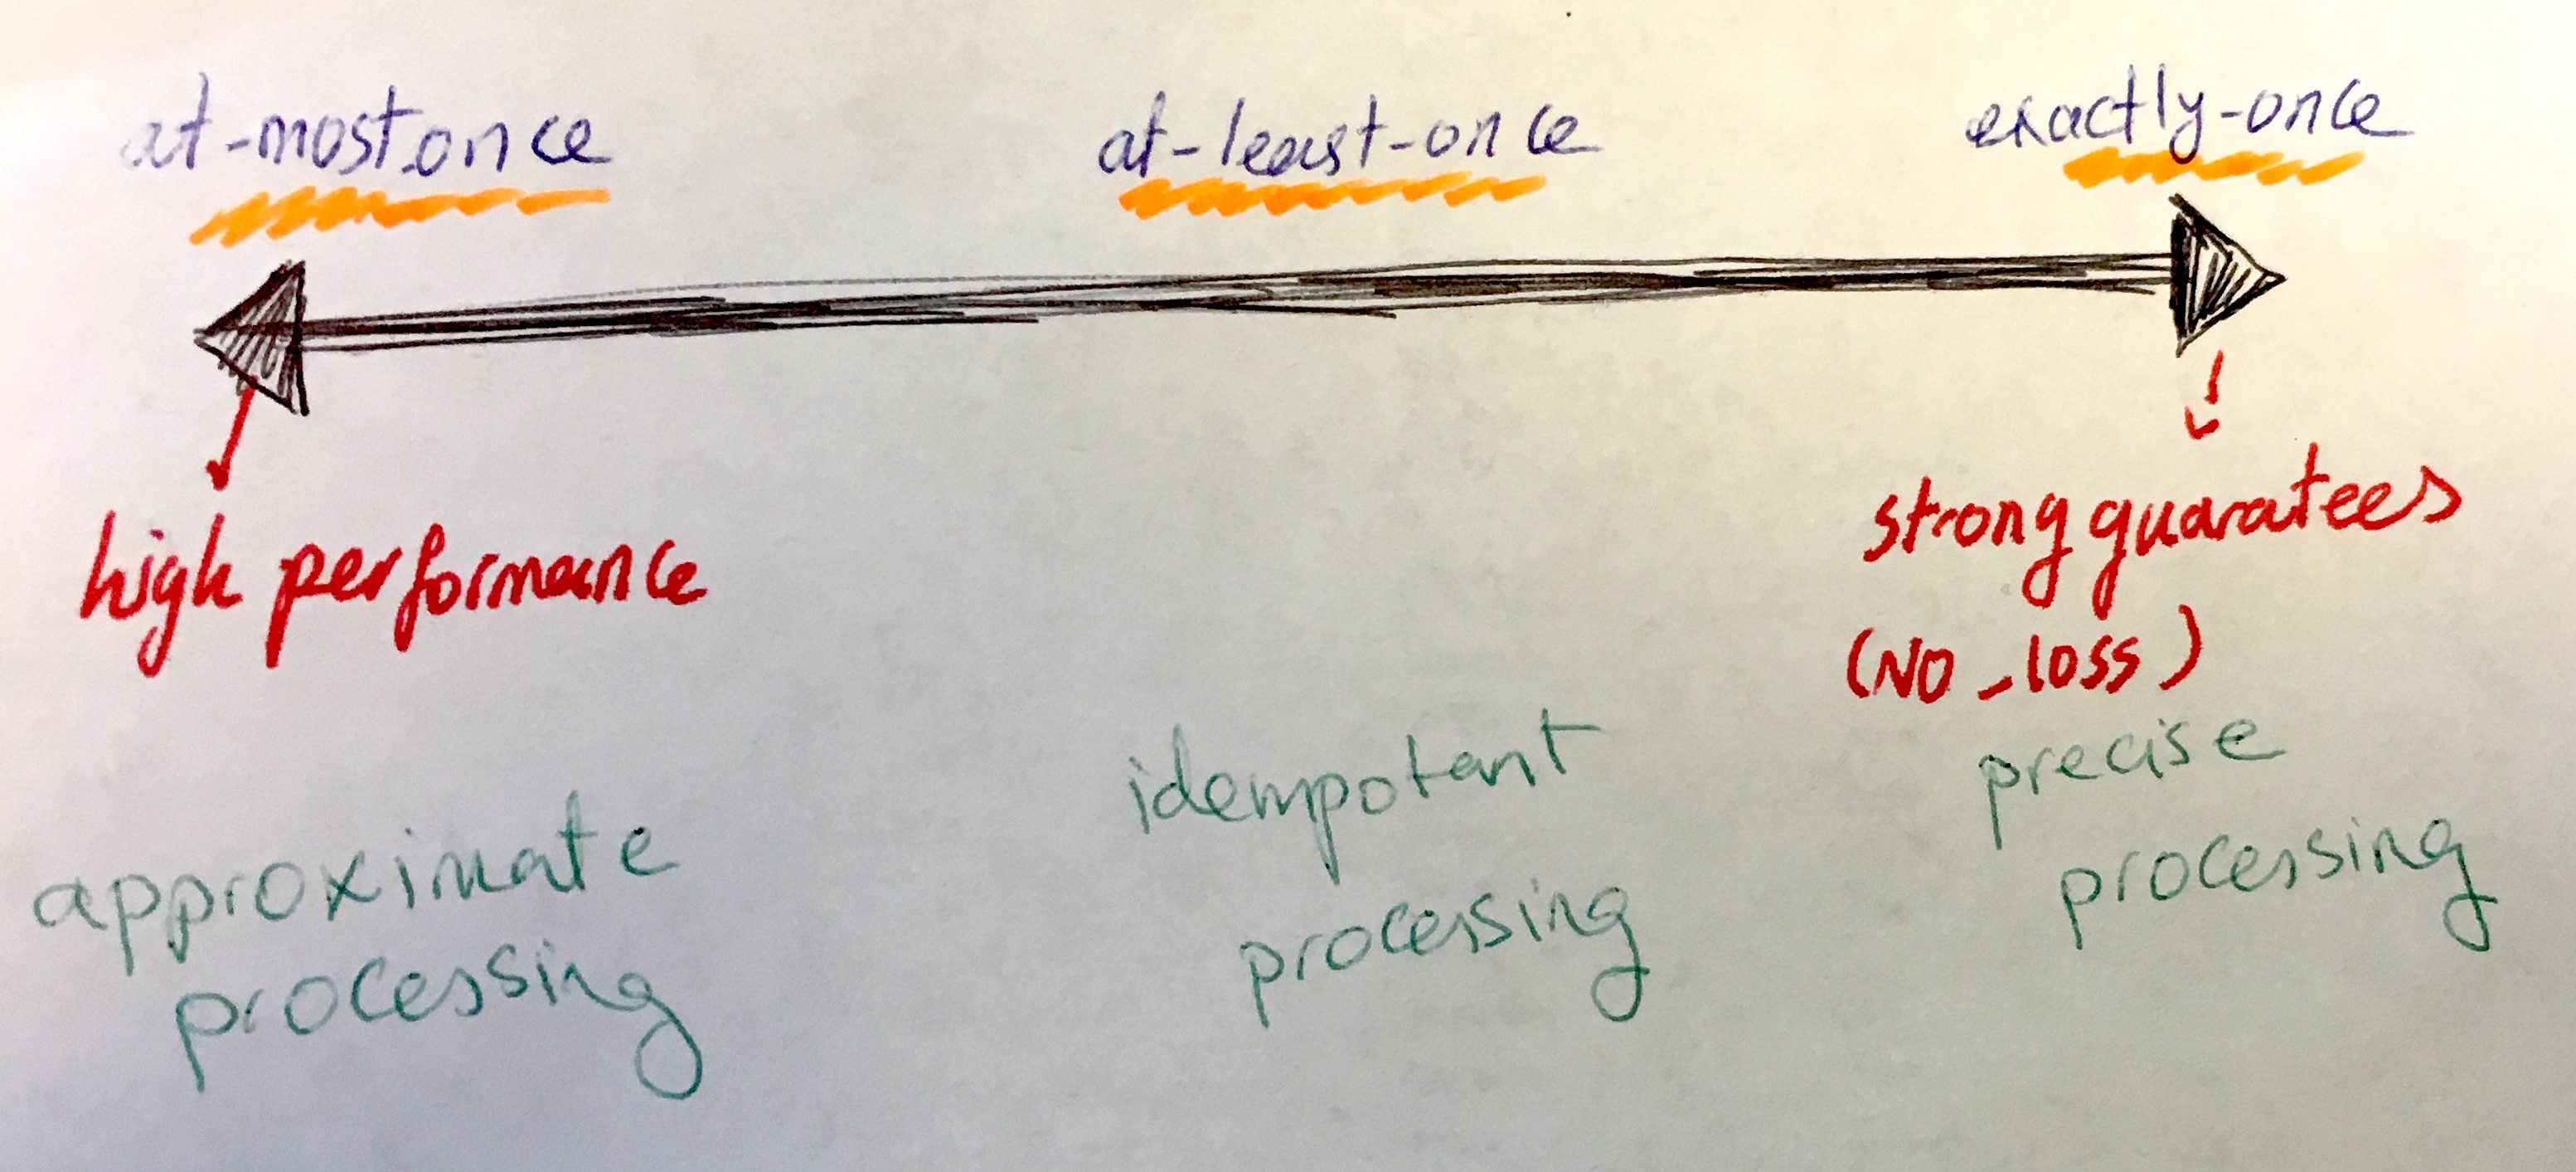
\includegraphics[width=0.45\linewidth]{guarantees.jpg}
	\caption{Spectrum of various failure properties and the trade-off among them.}
	\label{fig:failure}
\end{figure}

\begin{itemize}
	\item precise recovery:  \borrowed{hides the effects of a failure perfectly, except
		for some transient increase in processing latency, and is
		well-suited for applications that require the post-failure output
		be identical to the output without failure. Many financial
		services applications have such strict correctness requirements.}
	\item rollback recovery: \borrowed{ avoids information loss without guaranteeing
		precise recovery. The output produced after a failure
		is “equivalent” to, but not necessarily the same as, the
		output of an execution without failure. The output may also
		contain duplicate tuples. To avoid information loss, the system
		must preserve all the necessary input data for the backup
		server to rebuild (from its current state) the primary’s state at
		the moment of failure. Rollback recovery is thus appropriate
		for applications that cannot tolerate information loss but
		may tolerate imprecise output caused by the backup server
		reprocessing the input somewhat differently than the primary
		did. Example applications include those that monitor specific
		conditions (e.g., fire alarms, theft prevention through asset
		tracking). We show in Section 6 that this recovery guarantee
		can be provided more efficiently than precise recovery both
		in terms of runtime overhead and recovery speed.}
	\item gap recovery: \borrowed{ our weakest recovery guarantee, addresses
		the needs of applications that operate solely on the most recent
		information (e.g., sensor-based environment monitoring),
		where dropping some old data is tolerable for reduced
		recovery time and runtime overhead}
\end{itemize}


\noindent \textbf{\\Solutions \& trade-offs:}

\borrowed{ employs a different combination of redundant
	computation, checkpointing, and remote logging, they offer
	different tradeoffs between runtime overhead and recovery
	performance.
}
\begin{itemize}
	\item \borrowed{all following items borrowed!}
	\item amnesia, a lightweight scheme that provides
	\textbf{gap} recovery without any runtime overhead (Section 4).
	\item  passive standby and active standby, two
	process-pairs [4, 10] approaches tailored to stream processing.
	In passive standby, each primary server (a.k.a. node) periodically
	reflects its state updates to its secondary node. In
	active standby, the secondary nodes process all tuples in parallel
	with their primaries. 
	\item  propose upstream backup,
	an approach that significantly reduces runtime overhead compared
	to the standby approaches while trading off a small
	fraction of recovery speed. 
	
	Last two items can be both roll-back and precise recovery.
	
	\Fix{are there other approaches?}
\end{itemize}


\begin{table}[h]
	\tbl{Solutions to \Fix{XXX} and their trade-offs	\label{table:failure-summary}}{
		\tiny		
		\begin{tabular}{p{.15 \linewidth}|p{.3 \linewidth}|p{.3 \linewidth}|p{.1 \linewidth}}%
			
			\hline
			\rowcolor[HTML]{E0E0E0} 
			Solution	&Pros&Cons & Usecase
			\csvreader[head to column names]{tables/template-summary.csv}{}% use head of csv as column names
			{\\\hline\textbf{\csvcoli} & \csvcolii & \csvcoliii & \csvcoliv}% specify your coloumns here
			\\ \hline
		\end{tabular}	
	}
\end{table}


\noindent \textbf{\\Future Direction:}  
\section{Back Pressure Handling}
\section{Handling Stragglers}
\section{Summary of Building Blocks}
building-blocks-summary


\begin{table}[h]
	%\centering
	\tbl{Building Blocks used in most popular Stream Processing Engines.	\label{table:blocks-summary}}{
		%		\begin{tabular}{|p{.1 \linewidth}|p|p|p|p|p|p|p|p|p|p|p|p|}%
		\tiny
		%	\begin{tabular}{|p{.09 \linewidth}|p{.05 \linewidth}|p{.05 \linewidth}|p{.05 \linewidth}|p{.05 \linewidth}|p{.05 \linewidth}|
		%	p{.05 \linewidth}|p{.05 \linewidth}|p{.05 \linewidth}|p{.05 \linewidth}|p{.05 \linewidth}|p{.05 \linewidth}|p{.05 \linewidth}|}%
		
		\begin{tabular}{|p{.1 \linewidth}|p{.15 \linewidth}|p{.35 \linewidth}|p{.35 \linewidth}|}%
			
			\hline
			\rowcolor[HTML]{E0E0E0} 
			Feature	&Options	&Pros&Cons 
			%	bb & Storm & Heron & Trident & Samza & Spark & Millwheel & Flink & S4 & Flume & Streams & Borealis & Aurora 
			%	 \textbf{} & \textbf{} & \textbf{} % specify table head
			\csvreader[head to column names]{tables/building-blocks-summary.csv}{}% use head of csv as column names
			{\\\hline\textbf{\csvcoli} & \csvcolii & \csvcoliii &\csvcoliv }% specify your coloumns here
			\\ \hline
		\end{tabular}	
	}
\end{table}



% Please add the following required packages to your document preamble:
% \usepackage{multirow}


%%%%%%%%%% SYSTEMS %%%%%%%%%%%%%
\section{Big Data Processing Pipeline Architectures}
\section{Current Popular Stream Processing Systems}

\subsection{Storm}
\subsection{Heron}
\subsection{Samza}
\subsection{Spark Streaming}
\subsection{MillWheel}
\subsection{Flink}

\subsection{Building Blocks used in Modern systems}
\begin{table}[h]
	%\centering
	\tbl{Building Blocks used in most popular Stream Processing Engines.	\label{system-blocks}}{
%		\begin{tabular}{|p{.1 \linewidth}|p|p|p|p|p|p|p|p|p|p|p|p|}%
			\tiny
		%	\begin{tabular}{|p{.09 \linewidth}|p{.05 \linewidth}|p{.05 \linewidth}|p{.05 \linewidth}|p{.05 \linewidth}|p{.05 \linewidth}|
			%	p{.05 \linewidth}|p{.05 \linewidth}|p{.05 \linewidth}|p{.05 \linewidth}|p{.05 \linewidth}|p{.05 \linewidth}|p{.05 \linewidth}|}%
		
			\begin{tabular}{|p{.05 \linewidth}|p{.04 \linewidth}|p{.05 \linewidth}|p{.05 \linewidth}|p{.05 \linewidth}|p{.05 \linewidth}|
				p{.05 \linewidth}|p{.05 \linewidth}|p{.05 \linewidth}|p{.085 \linewidth}|p{.078 \linewidth}|p{.052 \linewidth}|p{.05 \linewidth}|}%
			
			\hline
			\rowcolor[HTML]{E0E0E0} 
				 &API &	Communication	& Guarantees &	Flexibility	&Inaccuracy Handling &	Distribution \& Scaling&	Fault Handling&	State Handling&	Reprocessing / Replayability	&Resource Management	& Back Pressure&	Processing Pipeline 
	%	bb & Storm & Heron & Trident & Samza & Spark & Millwheel & Flink & S4 & Flume & Streams & Borealis & Aurora 
		%	 \textbf{} & \textbf{} & \textbf{} % specify table head
			\csvreader[head to column names]{tables/system-blocks.csv}{}% use head of csv as column names
			{\\\hline\csvcoli & \csvcolii & \csvcoliii &\csvcoliv & \csvcolv & \csvcolvi &
			\csvcolvii & \csvcolviii & \csvcolix & \csvcolx   & \csvcolxi & \csvcolxii & \csvcolxiii}% specify your coloumns here
		\\ \hline
		\end{tabular}	
	}
\end{table}




%%%%%%%%%%% Future %%%%%%%%%%%%%
\section{Future of Stream: Remaining Challenges}





% Numbered Equation
%\begin{equation}
%\label{eqn:01}
%P(t)=\frac{b^{\frac{t+1}{T+1}}-b^{\frac{t}{T+1}}}{b-1},
%\end{equation}

% Algorithm
%\begin{algorithm}[t]
%\SetAlgoNoLine
%\KwIn{ss}
%\KwOut{ds}
%\Repeat{$FreNum_{\alpha} > -1$}{
%        \For{each node $\beta$ in $\alpha$'s two communication hops
%    }{
%     
%     \eIf{$Found$}{
%           $FreNum_{\alpha}$ = $index$\;
%         }{
%           $index$ ++\;
%     }      
%  }
%}
%\caption{Frequency Number Computation}
%\label{alg:one}
%\end{algorithm}


\section{Conclusions}


% Appendix
%\appendix
%\section*{APPENDIX}
%\setcounter{section}{1}
%\appendixhead{ZHOU}
%
%% Acknowledgments
%\begin{acks}
%	\cite{Editor00}
%\end{acks}

% Bibliography
\bibliographystyle{ACM-Reference-Format-Journals}
\bibliography{references.bib}
                             % Sample .bib file with references that match those in
                             % the 'Specifications Document (V1.5)' as well containing
                             % 'legacy' bibs and bibs with 'alternate codings'.
                             % Gerry Murray - March 2012

% History dates
%\received{February 2007}{March 2009}{June 2009}

% Electronic Appendix
%\elecappendix

\medskip

%\section{This is an example of Appendix section head}


%\section{Appendix section head}

\end{document}
% End of v2-acmsmall-sample.tex (March 2012) - Gerry Murray, ACM


